Consider a two-species predator-prey model in which one species preys on another.
Examples in the natural world include sharks and fish, lynx and snowshoe hares, and ladybirds and aphids.
A very simple differential equation—first used by \emph{Volterra} in 1926 and known as the \emph{Lotka-Volterra model}.\\
The Equations are given by
\begin{equation}{\label{eq:pp}}
	\begin{aligned}
		\dot{x}=x(\alpha-cy)\\
		\dot{y}=y(\gamma x-\delta)
	\end{aligned}
\end{equation}
where $\alpha, c, \gamma, and\ \delta$ are all positive constants, with $x(t)$ and $y(t)$ representing the scaled population of prey and predator, respectively, and t is measured in years.\\
Physical Meaning:
\begin{itemize}
	\item The term $\alpha x$ represents the growth of the population of prey in the absence of any predators. This is obviously a crude model; the population of a species cannot increase forever.
	\item The terms $-cxy$ and $+\gamma xy$ represent species interaction. The population of prey suffers and predators gain from the interaction.
	\item The term $-\delta y$ represents the extinction of predators in the absence of prey.
\end{itemize}
Fixed points of equation (\ref{eq:pp}) are
\begin{equation}
	O=(0,0) \quad and \quad P=\left(\frac{\delta}{\gamma},\frac{\alpha}{c}\right)
\end{equation}
Linearize by finding the Jacobian matrix.
\begin{equation}
	J=
	\begin{pmatrix}
		\alpha-cy&-cx\\\gamma y&-\delta+\gamma x
	\end{pmatrix}\quad\rightarrow\quad
	J_O=
	\begin{pmatrix}
		\alpha&0\\
		0&-\delta
	\end{pmatrix}\quad
	J_P=
	\begin{pmatrix}
		0&-c\delta/\gamma\\
		\gamma\alpha/c&0
	\end{pmatrix}
\end{equation}
The critical point at the origin is a saddle point, and the stable and unstable manifolds lie along the axes.
The stable manifold lies on the positive $y-$axis, and the unstable manifold lies on the $x-$axis.
The critical point at $P$ is not hyperbolic, and so Hartman’s Theorem cannot be applied. System (\ref{eq:pp}) has solution curves (the differential equation is separable) given by $x^\delta y^\alpha e^{-\gamma x}e^{-cy}=K$, where $K$ is a constant.
These solution curves may be plotted in the phase plane. A phase portrait is shown in Figure (\ref{fig:pp}).
\begin{figure}[H]
	\centering
	\begin{subfigure}{0.45\linewidth}
		\raggedleft
		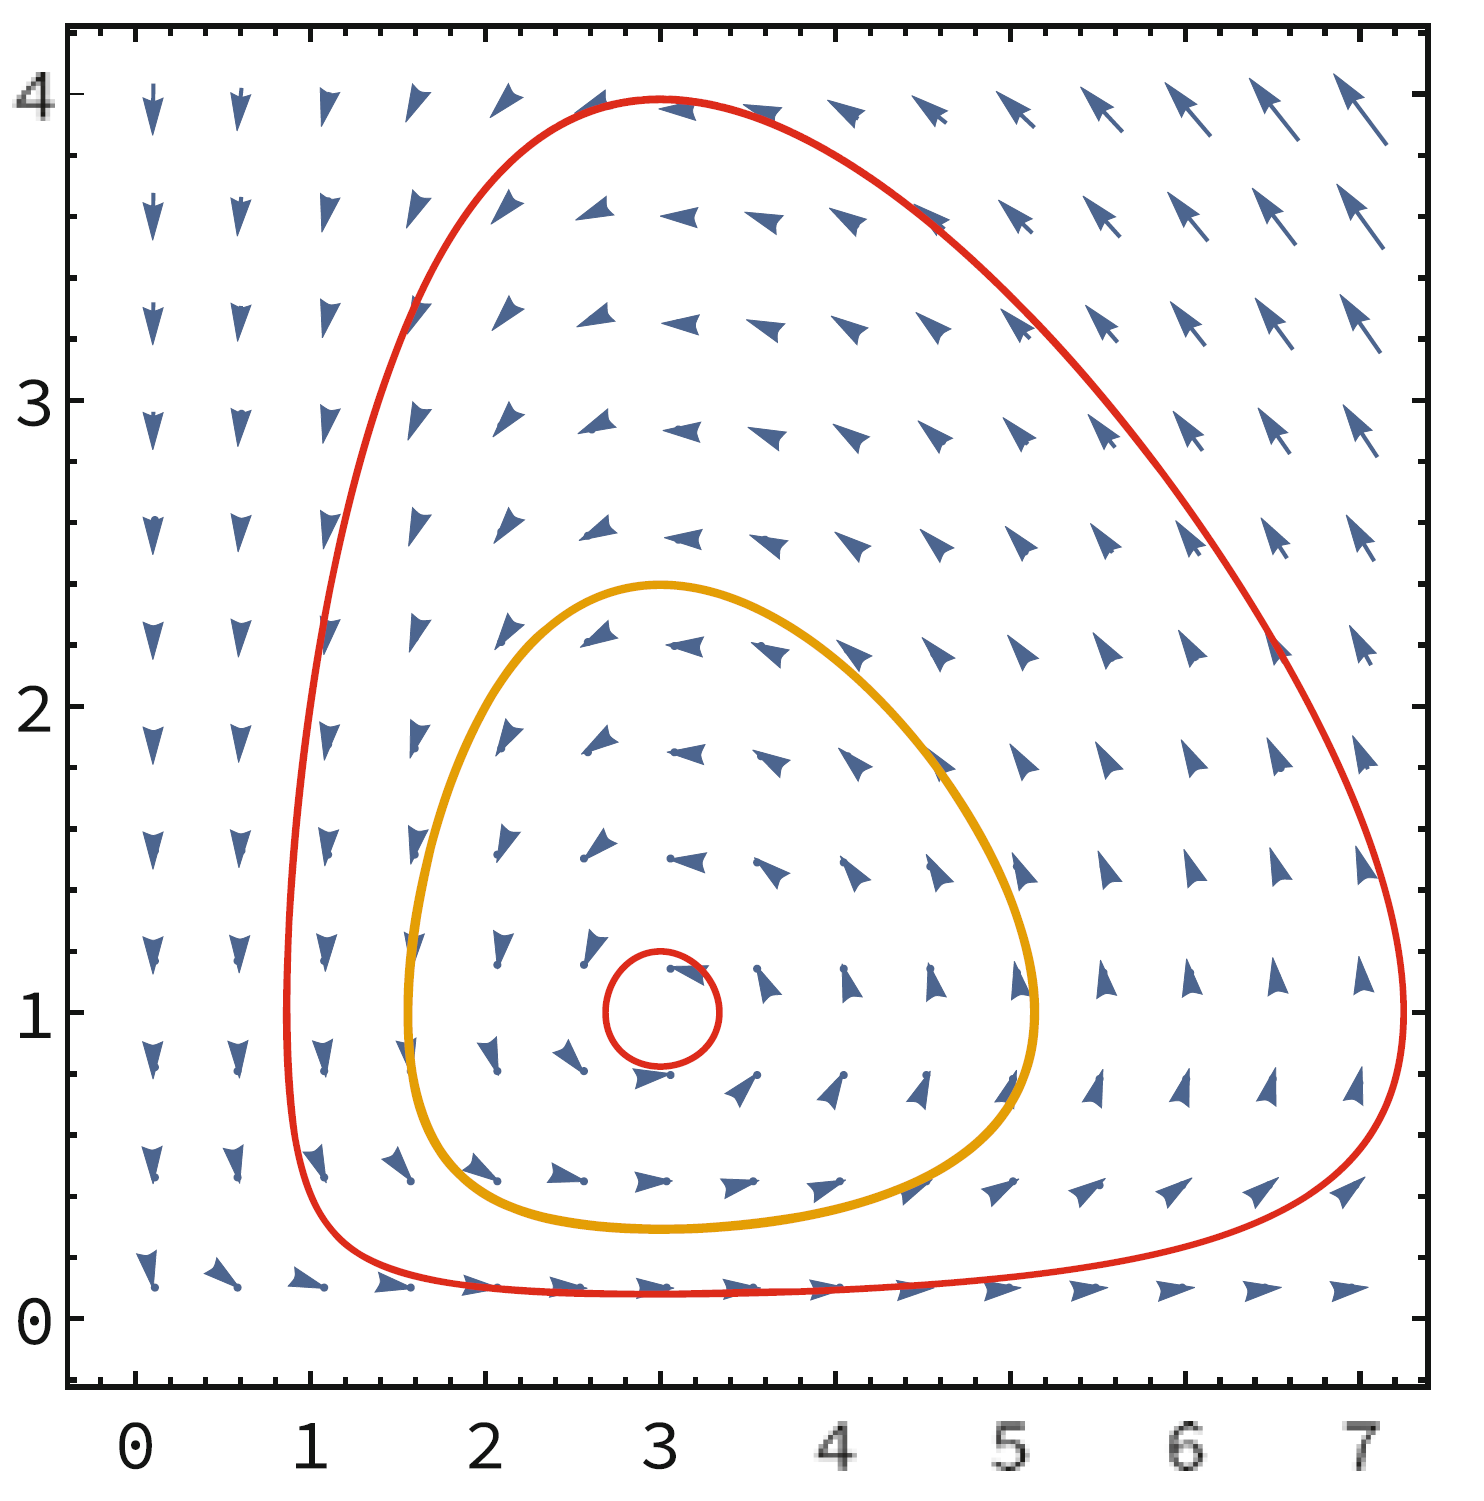
\includegraphics[width=0.54\linewidth]{pp1.png}
		\caption{A phase portrait for the Lotka Volterra model.}
		\label{fig:pp}
	\end{subfigure}
	\vline
	\begin{subfigure}{0.45\linewidth}
		\raggedright
		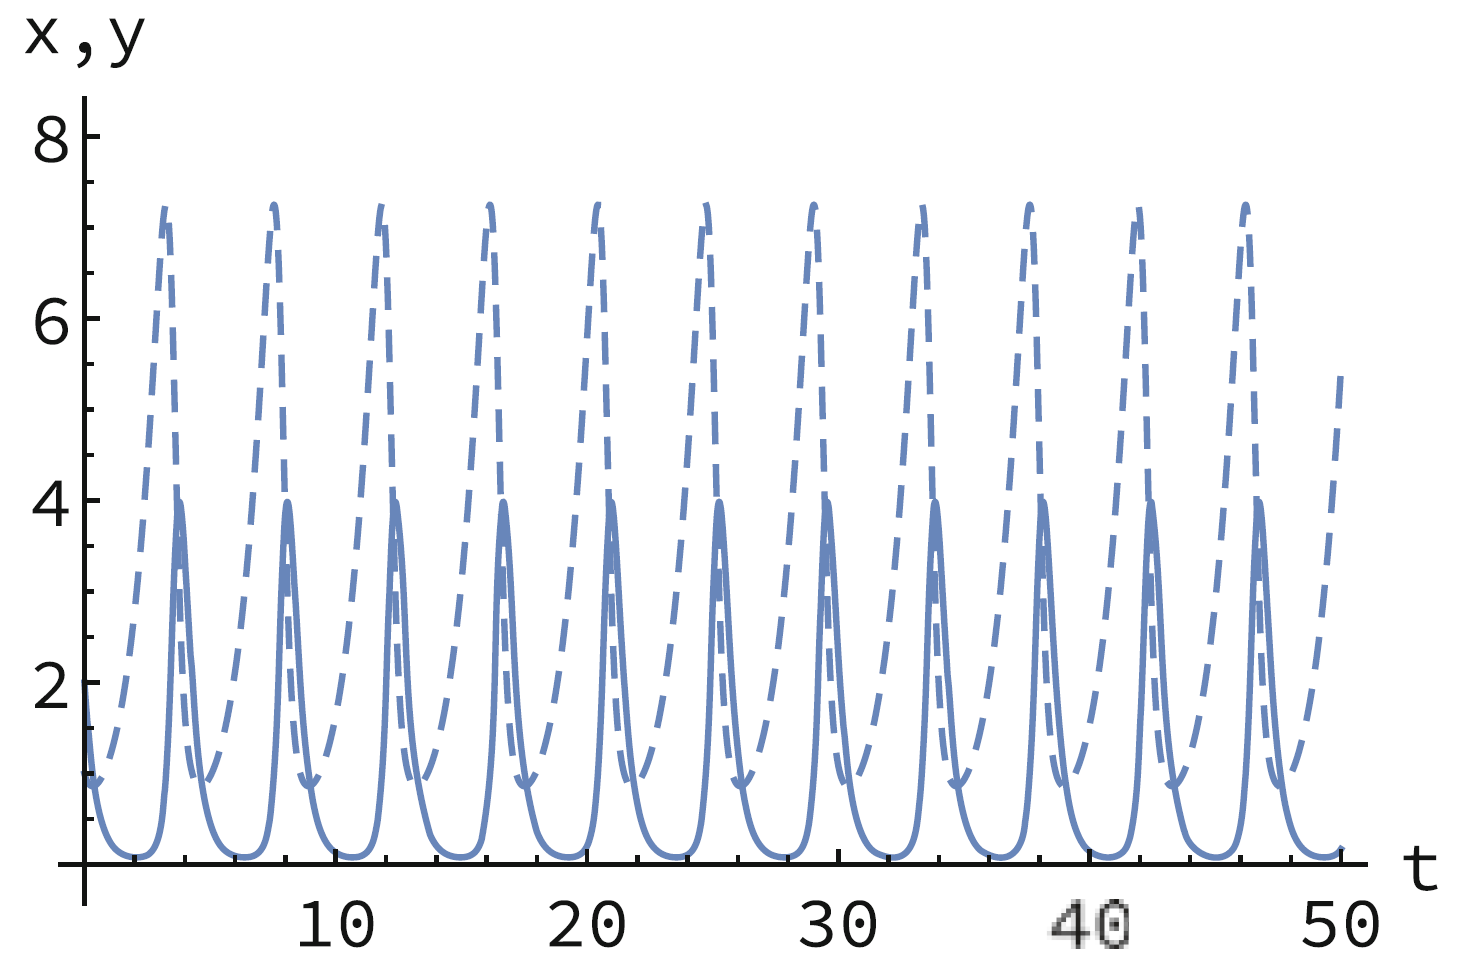
\includegraphics[width=0.7\linewidth]{pp2.png}
		\caption{Time series plots, periodic behavior of the prey and predators for one set of initial conditions, namely $x(0)=1, y(0)=2$. The population of prey is shown as the dashed curve and the population of predator is a solid curve.}
		\label{fig:pp2}
	\end{subfigure}
	\caption{}
\end{figure}
The population fluctuations can also be represented in the tx and ty planes.
The graphs shown in Figure (\ref{fig:pp}) show how the populations of predator and prey typically oscillate.
Note that the oscillations are dependent on the initial conditions. In Figure (\ref{fig:pp2}), the period of both cycles is about $5$ years.
\emph{Different} sets of {\textbf{initial conditions}} can give solutions with \emph{different} {\textbf{amplitudes}}.\\
Consider the trajectory passing through the point $(1, 1)$ in Figure (\ref{fig:pp}).
At this point, the ratio of predators to prey is relatively high; as a result, the population of predators drops.
The ratio of predators to prey drops, and so the population of prey increases.
Once there are lots of prey, the predator numbers will again start to increase. The resulting cyclic behavior is repeated over and over and is shown as the largest closed trajectory in Figure (\ref{fig:pp}).\\
If small perturbations are introduced into system (\ref{fig:pp}) to model other factors, for example, then the qualitative behavior changes.
The periodic cycles can be destroyed by adding small terms into the right-hand sides of system (\ref{fig:pp}).
The system is said to be {\textbf{structurally unstable}}.\\	
In 1975, \emph{Holling and Tanner} constructed a system of differential equations whose solutions have the same amplitudes in the long term, no matter what the initial populations.